\chapter{Clustering con restricciones}\label{ch:Clustering con restricciones}

El objetivo de este epígrafe es definir los conceptos relacionados con el clustering con restricciones, así como dar ejemplos de su aplicación y destacar los beneficios y problemas que presenta su uso. A tal fin tomamos como referencia principal el trabajo de Ian Davidson y Sugato Basu (2007) \cite{Survey:2007} entre otros.

\section{Motivación para el clustering con restricciones}

Tal y como hemos estudiado en epígrafes anteriores, los métodos de clustering no supervisado son útiles para dotar de estructura a datos referentes a un área concreta. Un ejemplo de ello lo encontramos en la clasificación de textos; Cohn et al. (2003) \cite{Cohn:2003} afrontan un problema propuesto por Yahoo!, que consiste en, dada una gran cantidad de documentos de texto, agruparlos según una taxonomía en la que los documentos con temáticas similares se encuentren cercanos. Para ello, los métodos de clustering no supervisado resultan de utilidad, ya que la información sobre el problema de la que se dispone inicialmente es limitada. Sin embargo, Wagstaff et al. (2001) mostraron que aplicando clustering no supervisado a ciertos problemas, como el de agrupar datos de GPS de forma que los clusters definan los carriles de una vía, no se obtienen resultados significativos, pues los clusters obtenidos distan mucho de la forma alargada que se esperaría como resultado. Para atajar el problema, introdujeron en el clustering un nuevo elemento, las restricciones a nivel de instancia, que permitían incluir conocimiento sobre los clusters que guiarían los métodos de clustering para obtener los resultados esperados. Bastaba con indicar que los carriles de la vía por la que circulan los vehículos miden cuatro metros de ancho, y por tanto cualquier vehículo que se encuentre a una distancia mayor de 4 metros de otro, en dirección perpendicular a la del desplazamiento, debe ser ubicado en un cluster diferente.

Nos situamos entonces en un nuevo escenario: es posible incorporar información adicional al proceso de clustering, además de la contenida en el propio conjunto de datos, para guiarlo en la formación de la partición y obtener resultados mas precisos. Esto sitúa al clustering con restricciones en el marco del aprendizaje semisupervisado, a diferencia de los métodos de clustering tradicionales que se enmarcan en el área del clustering no supervisado. 

\section{Definición de las restricciones}

El nuevo tipo de  información que incorporamos al clustering viene dado en forma de restricciones a nivel de instancia, esto es, especificar si dos instancias del conjunto de datos deben estar en el mismo cluster, o, por el contrario, deben estar en clusters separados.

A las restricciones que indican que dos puntos deben ser situados en el mismo cluster se las denomina Must-link, y se notan por $ML(x,y)$, donde $x$ e $y$ son dos instancias del conjunto de datos. De manera similar, a las restricciones que especifican lo contrario se las denomina Cannot-link, y se notan por $CL(x,y)$. \cite{WagstaffCardie:2000}

Aunque pueden parecer simples, las restricciones definidas de la anterior forma poseen propiedades interesantes. Las Restricciones de tipo Must-link son un ejemplo de relación de equivalencia, y por tanto son simétricas, reflexivas y transitivas, formalizando:

\begin{observacion}
	\textbf{Las restricciones de tipo ML son transitivas.} Sean $CC_i$ y $CC_j$ componentes conexas, conectadas mediante restricciones $ML$, y sean $x$ e $y$ dos instancias en $CC_i$ y $CC_j$ respectivamente. Entonces $ML(x,y): x \in CC_i, y \in CC_j \rightarrow ML(a,b) \forall a,b: a\in CC_i, b \in CC_j$. \cite{Survey:2007}
\end{observacion}

\begin{observacion}
	\textbf{Las restricciones de tipo CL pueden ser (encadenadas).} Sean $CC_i$ y $CC_j$ componentes conexas, conectadas mediante restricciones $ML$, y sean $x$ e $y$ dos instancias en $CC_i$ y $CC_j$ respectivamente. Entonces $CL(x,y): x \in CC_i, y \in CC_j \rightarrow CL(a,b) \forall a,b: a\in CC_i, b \in CC_j$. \cite{Survey:2007}
\end{observacion}

Un claro ejemplo de uso de las restricciones lo encontramos en casos de aplicación de clustering en los que existen restricciones en cuanto a las medidas de distancia, como sucedía en el supuesto de los datos GPS. Así, si queremos que las instancias que forman dos clusters estén separadas por una distancia mayor o igual a $\delta$, basta con establecer restricciones de tipo ML entre todas aquellas instancias cuya distancia sea menor que $\delta$. 
De manera similar, si queremos que el diámetro de los clusters sea como mucho $\epsilon$, debemos establecer un conjunto de restricciones de tipo CL entre todas aquellas instancias que se encuentren a una distancia mayor que $\epsilon$. La figura \ref{fig:figure4} muestra una representación gráfica de estos dos tipos de restricciones.

\begin{figure}[!h]
	\centering
	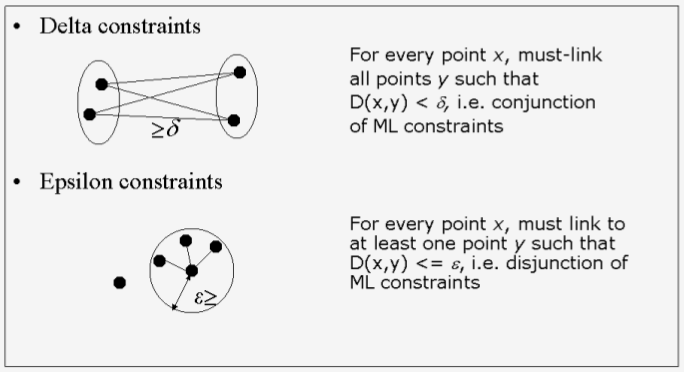
\includegraphics[scale=0.45]{imagenes/c3/RestriccionesDeltaEpsilo.png} 
	\caption{Restricciones de tipo delta y epsilon. \cite{Survey:2007}}\label{fig:figure4}
\end{figure}


\section{Uso de las restricciones}

Mientras que el aprendizaje completamente supervisado implica conocer la etiqueta asociada a cada instancia, en el aprendizaje semisupervisado solo se dispone de un subconjunto de instancias etiquetadas. Por otra parte, en gran cantidad de dominios la información disponible se refiere a relaciones entre instancias, y no a la clase concreta a la que pertenecen las mismas. Es más, en montajes de clustering interactivo, un usuario no experto en el dominio del problema podrá, probablemente, aportar información en forma de restricciones de tipo \acf{ML} y \acf{CL} \cite{Cohn:2003}\cite{DavidsonRavi:2007}, antes que aportar información sobre a qué clase concreta pertenecen ciertas instancias.

Habitualmente, las restricciones se incluyen en los problemas de clustering de dos maneras. Pueden ser empleadas para modificar la regla de asignación de instancias a clusters del método en cuestión, de forma que la solución satisfaga el máximo número de restricciones posible. Alternativamente, cabe la posibilidad de entrenar la función de distancia empleada por el método en base a las restricciones, ya sea antes o durante la aplicación del mismo. En cualquier caso, la fase incialización puede tomar en consideración las restricciones, de forma que las instancias asociadas con restricciones \acf{ML} serán situadas en el mismo cluster, y aquellas entre las que exista una restricción \acf{CL}, quedarán en clusters diferentes. Basándonos en esta distinción, identificamos dos maneras de aproximar el problema, las basadas en restricciones (\textit{constraint-based}), y las basadas en distancias (\textit{distance-based}).

\subsection{Métodos basados en restricciones}

En los métodos basados en restricciones, el propio método de clustering es modificado de manera que la información disponible se emplea para sesgar la búsqueda y obtener una partición de los datos apropiada.

Existen dos modelos de métodos basados en restricciones: (1) aquellos que fuerzan el cumplimiento de las restricciones, e intentan encontrar la mejor asignación posible que no inflija ninguna de ellas \cite{Wagstaff:2001b}\cite{DavidsonRavi:2005b}, y (2) las que hacen una interpretación relajada de las restricciones \cite{Basu:2004}\cite{Seagal:2003}\cite{DavidsonRavi:2005a}\cite{Law:2005}, permitiéndose incumplir un número mínimo de ellas para optimizar la función objetivo, de esta manera surge un compromiso entre el número de restricciones incumplidas y el valor de la función objetivo. Existen diversas técnicas para obtener una partición atendiendo a las restricciones:

\begin{itemize}
	
	\item Modificar la función objetivo de manera que incluya una penalización por incumplir restricciones. \cite{Demiriz:1999} \cite{DavidsonRavi:2005a}
	
	\item Agrupar instancias con información adicional obtenida de una distribución condicional en un espacio auxiliar. \cite{SinkkonenKaski:2000}
	
	\item Forzar el cumplimiento de todas las restricciones modificando la regla de asignación del método. \cite{Wagstaff:2001b}
	
	\item Inicializando los clusters e base a restricciones inferidas del conjunto de instancias etiquetadas.\cite{Basu:2002}
	
\end{itemize}

La figura \ref{fig:figure5} muestra un conjunto de datos junto a sus restricciones asociadas, la \ref{fig:figure6} propone un posible agrupamiento que satisface todas las restricciones.

\begin{figure}[bth]
	\myfloatalign
	{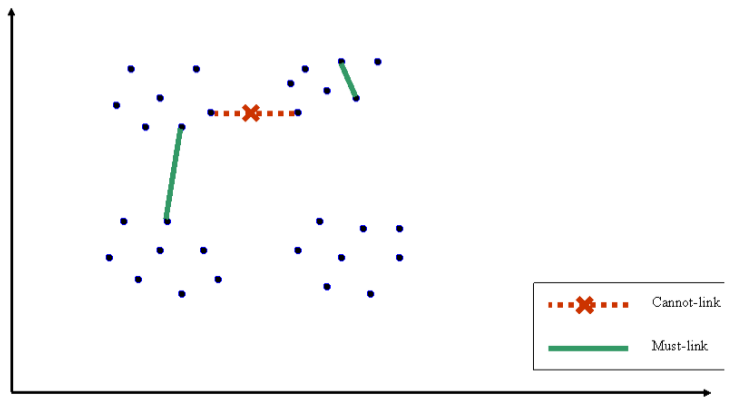
\includegraphics[width=.6\linewidth]{imagenes/c3/InputInstancesAndConst1}
	\caption{Restricciones sobre un conjunto de datos. \cite{Survey:2007}} \label{fig:figure5}
	}
	{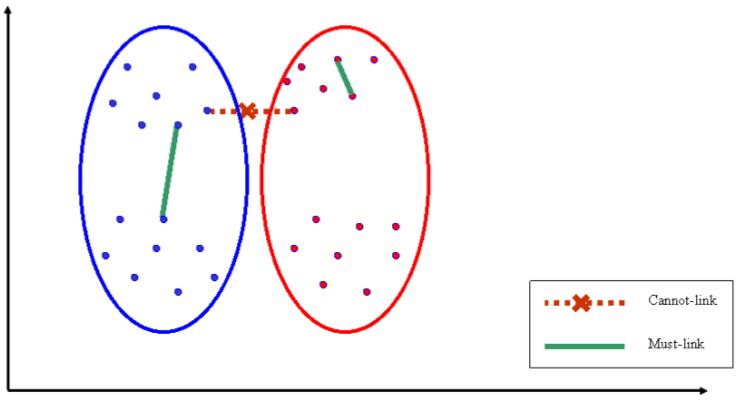
\includegraphics[width=.6\linewidth]{imagenes/c3/ClusteringSatAll}
	\caption{Clustering que satisface todas las restricciones. \cite{Survey:2007}} \label{fig:figure6}
	}
\end{figure}

\subsection{Métodos basados en distancia}

En las aproximaciones basadas en distancias, se emplean métodos de clustering clásicos que hagan uso de una medida de distancia, de forma que dicha medida se modifica para que tenga en consideración las restricciones. En este contexto, satisfacer las restricciones significa que las instancias relacionadas con restricciones \acf{ML} se sitúan juntas en el espacio, y las relacionadas mediante \acf{CL} se encuentran separadas.

La figura \ref{fig:figure8} muestra un posible agrupamiento basado en una métrica aprendida a partir de las restricciones especificadas en la figura \ref{fig:figure7}. Cabe destacar que en la figura \ref{fig:figure8} el espacio en el que se encuentran los datos ha sido comprimido en el eje vertical y ensanchado en el eje horizontal para ajustarlo a la métrica de distancia aprendida.

\begin{figure}[bth]
	\myfloatalign
	{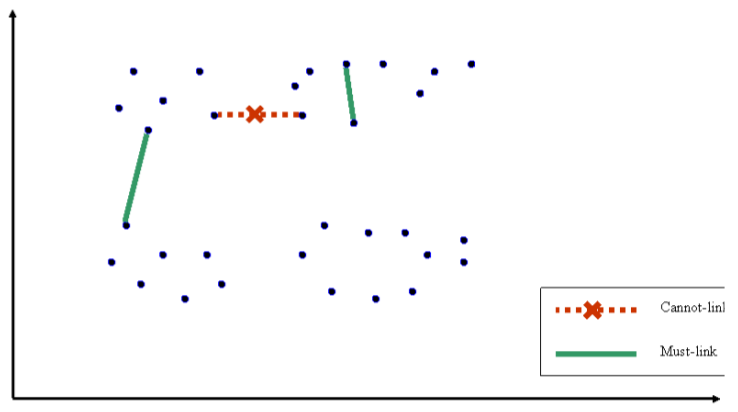
\includegraphics[width=.6\linewidth]{imagenes/c3/InputInstancesAndConst2}
	\caption{Restricciones sobre un conjunto de datos. \cite{Survey:2007}} \label{fig:figure7}
	}
	{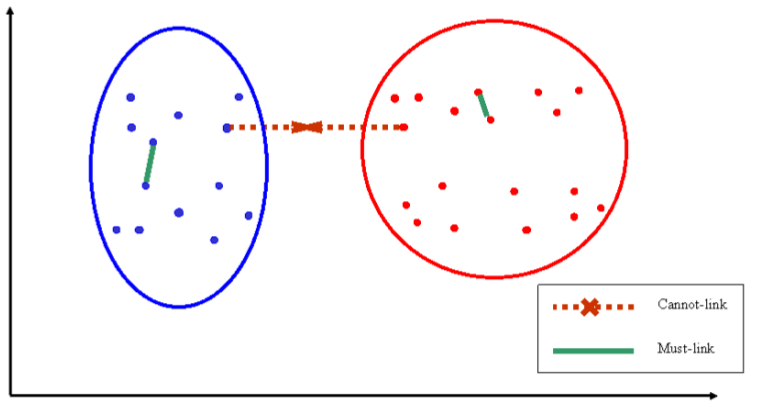
\includegraphics[width=.6\linewidth]{imagenes/c3/MetricaAprendida}
	\caption{Clustering basado en métrica aprendida en base a las restricciones. \cite{Survey:2007}} \label{fig:figure8}
	}
\end{figure}

\section{Aplicaciones del clustering con restricciones} 

Este epígrafe muestra algunos casos de aplicación en los que el clustering con restricciones ha resultado ser una herramienta más útil que el clustering no supervisado. Para cada caso analizaremos como se obtuvieron las restricciones y como estas mejoran los resultados en el clustering resultante. 

\subsection{Aplicaciones en análisis de imágenes}

La figura \ref{fig:figure9} muestra un extracto del conjunto de datos de caras de  \acf{CMU}, en el que la tarea es agrupar caras en base a diferentes criterios. En este caso, el objetivo es agrupar las caras según su orientación, es decir, las caras con la misma orientación deberán estar en el mismo cluster.

\clearpage

\begin{figure}[bth]
	\myfloatalign
	\subfloat[Caras de perfil]
	{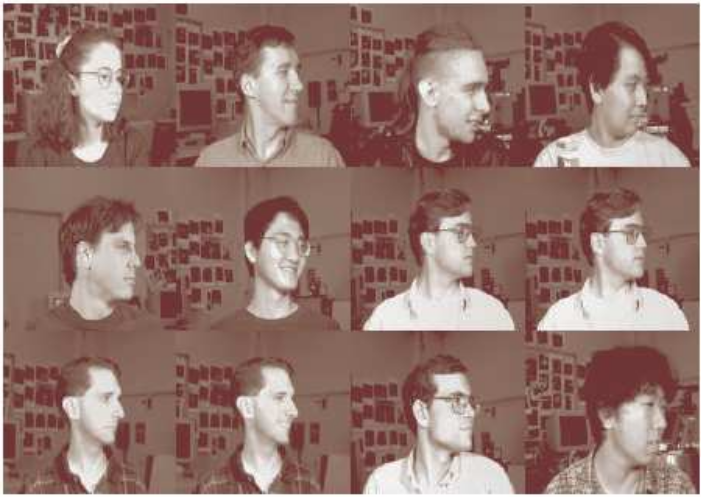
\includegraphics[width=.3\linewidth]{imagenes/c3/AnalisisImagenes/Caras1}} \quad
	\subfloat[Caras de frente.]
	{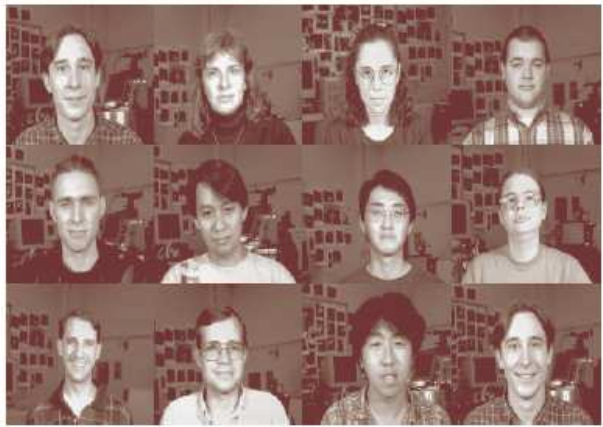
\includegraphics[width=.3\linewidth]{imagenes/c3/AnalisisImagenes/Caras3}} \quad
	\subfloat[Caras hacia arriba.]
	{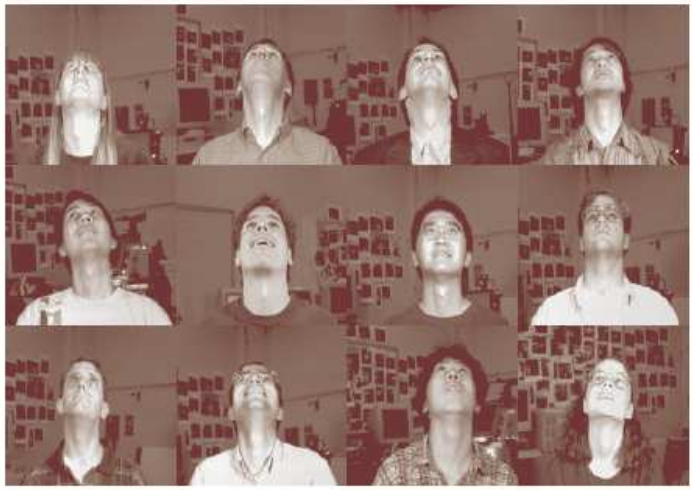
\includegraphics[width=.3\linewidth]{imagenes/c3/AnalisisImagenes/Caras2}} \quad
	\caption{Caras de la base de datos de  \ac{CMU}. \cite{Survey:2007}}\label{fig:figure9}
\end{figure}

El método empleado para extraer las restricciones es uno de los más populares en la literatura: establecer el número de clusters de la partición resultado igual al número de clases en la base de datos, y generar las restricciones a partir de un subconjunto de instancias etiquetadas, esto es, si dos instancias tiene diferentes etiquetas, establecer una restriccion \acf{CL} entre ellas, en caso contrario una de tipo \acf{ML}. De esta forma, entre las imágenes mostradas en la figura \ref{fig:figure10} se establecen restricciones \acf{CL}, ya que, aunque pertenecen a la misma persona, no presentan la misma orientación.

\begin{figure}[bth]
	\myfloatalign
	{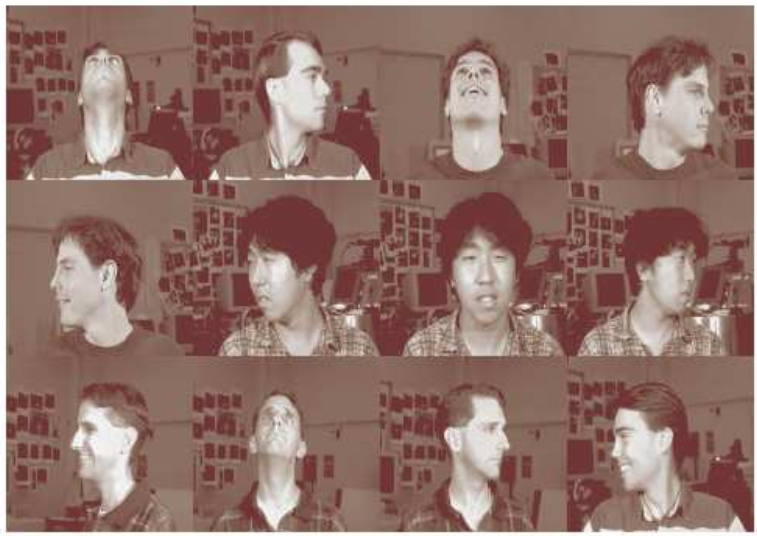
\includegraphics[width=.35\linewidth]{imagenes/c3/AnalisisImagenes/CarasDifOr1}} \quad
	{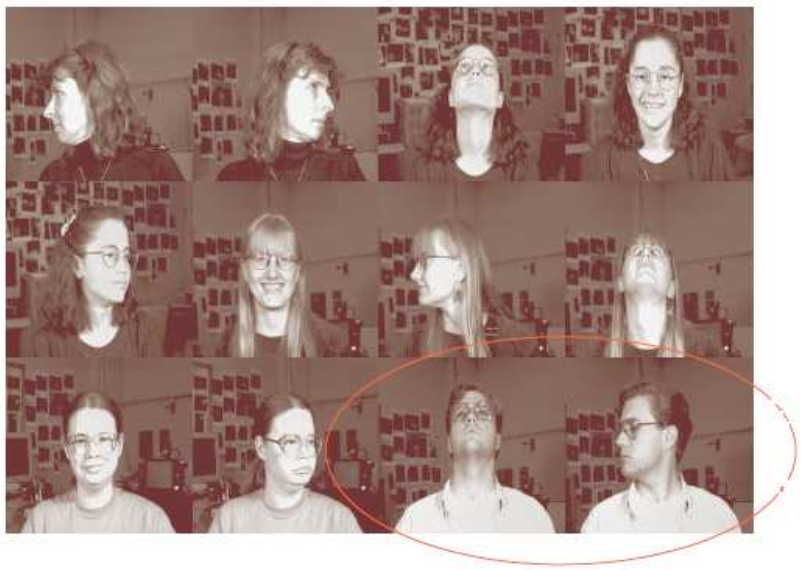
\includegraphics[width=.35\linewidth]{imagenes/c3/AnalisisImagenes/CarasDifOr2}}
	\caption{Restricciones de tipo \ac{CL} entre caras de la misma persona.  \cite{Survey:2007}}\label{fig:figure10}
\end{figure}

En la figura \ref{fig:figure11} se muestra otro conjunto de datos de imágenes sobre el que se aplican técnicas de clustering con restricciones. En este caso, la tarea es realizar reconocimiento de objetos para incorporar el método al sistema de navegación del robot Aibo \cite{DavidsonRavi:2005a}. Para ello se emplean restricciones de distancia de tipo $\delta$ y $\epsilon$ como las descritas en la figura \ref{fig:figure4}, de esta manera se consiguen clusters bien diferenciados y por tanto útiles para las tareas de búsqueda de caminos que el robot realiza durante la navegación.

\begin{figure}[bth]
	\myfloatalign
	\subfloat[Imagen original]
	{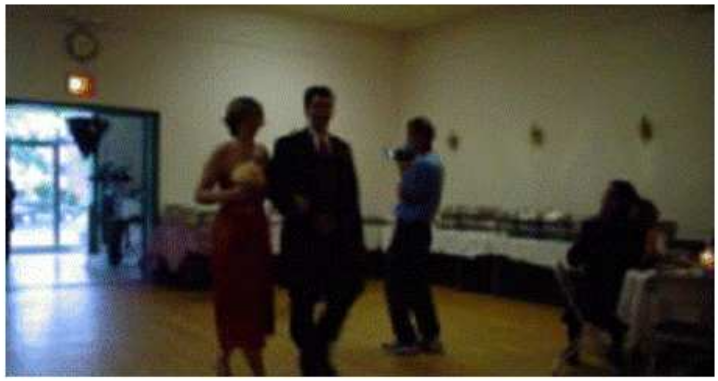
\includegraphics[width=.3\linewidth]{imagenes/c3/AnalisisImagenes/Aibo1}} \quad
	\subfloat[Clustering sin restricciones]
	{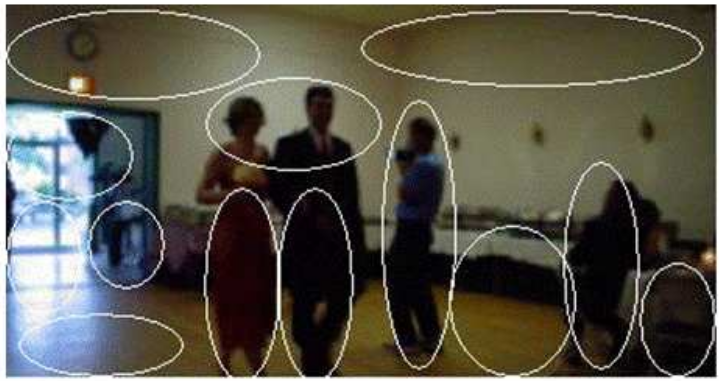
\includegraphics[width=.3\linewidth]{imagenes/c3/AnalisisImagenes/Aibo2}} \quad
	\subfloat[Clustering con restricciones]
	{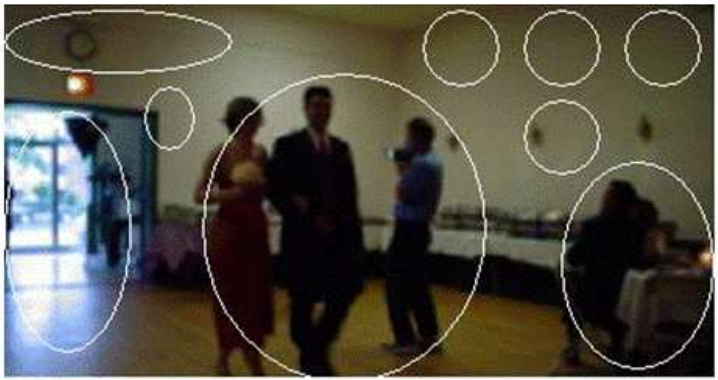
\includegraphics[width=.3\linewidth]{imagenes/c3/AnalisisImagenes/Aibo3}} \quad
	\caption{Método de clustering empleado en el sistema de navegación del robot Aibo. \cite{Survey:2007}\cite{DavidsonRavi:2005a}}\label{fig:figure11}
\end{figure}

\subsection{Aplicaciones en análisis de vídeos}

Las bases de datos de video son uno de los ejemplos en los que las restricciones pueden ser generadas directamente desde el dominio de datos, especialmente disponiendo de datos espacio-temporales sobre el vídeo \cite{Yan:2004}. En datos temporalmente sucesivos es posible establecer restricciones de tipo \acf{ML} entre grupos de píxeles de fotogramas (\textit{frames}) cercanos en el tiempo. Esto es especialmente útil cuando la tarea es implementar reconocimiento de objetos basado en clustering y segmentación. También es posible añadir restricciones \acf{CL} a clusters localizados en el mismo fotograma, ya que existe una baja probabilidad de que estén asociados al mismo objeto. De hecho, en el dominio asociado a problemas de análisis de vídeo existen gran variedad métodos de extracción de restricciones \cite{Yan:2004}, la figura \ref{fig:figure12} muestra algunos ejemplos.  

\begin{figure}[bth]
	\myfloatalign
	\subfloat[]
	{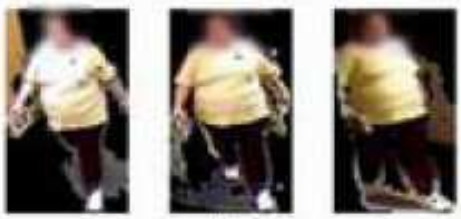
\includegraphics[width=.4\linewidth]{imagenes/c3/Videos/VideoA}}
	\quad
	\subfloat[]
	{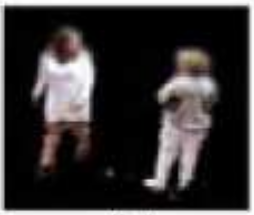
\includegraphics[width=.225\linewidth]{imagenes/c3/Videos/VideoB}} \quad
	\subfloat[]
	{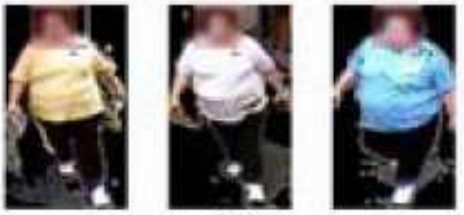
\includegraphics[width=.4\linewidth]{imagenes/c3/Videos/VideoC}}
	\quad
	\subfloat[]
	{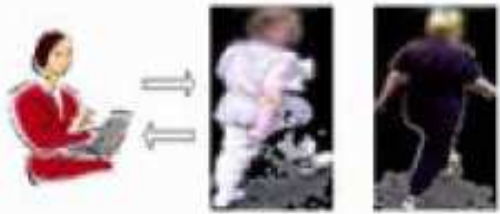
\includegraphics[width=.4\linewidth]{imagenes/c3/Videos/VideoD}}
	\caption{Diferentes tipos de restricciones en datos de video. \cite{Yan:2004} \cite{Survey:2007}}\label{fig:figure12}
\end{figure}

En la figura \ref{fig:figure12}, la imagen (a) corresponde a restricciones extraídas del seguimiento de una persona durante un periodo de tiempo, la (b) corresponde a restricciones espaciales que asocian dos objetos localizados en el mismo fotograma, la imagen (c) corresponde a restricciones obtenidas mediante reconocimiento facial y la (d) a las proporcionadas por el usuario.

Disponiendo de tantos métodos para extraer restricciones, cabe plantearse, ¿qué sucede si se establecen demasiadas restricciones? ¿Hace esto que el problema esté sobrerestringido? En epígrafes posteriores abordaremos estas cuestiones.

\subsection{Aplicaciones en genética}

En clustering de genes basado en microarrays, los genes vienen representados por su perfil de expresión en diferentes experimentos y agrupados empleando diferentes métodos, en este caso métodos de clustering con restricciones. La  figura \ref{fig:figure13} muestra un ejemplo, se trata de restricciones de tipo \acf{ML} se establecen entre genes en base a los datos de co-ocurrencia almacenados en la base de datos de interacciones de proteínas, que contiene información sobre qué genes (y sus proteínas asociadas) están presentes en los mismos procesos celulares \cite{Xenarios:2001}. Esta información puede ser empleada para mejorar los resultados que proporcionan los métodos de clustering. \cite{Seagal:2003}

\begin{figure}[!h]
	\centering
	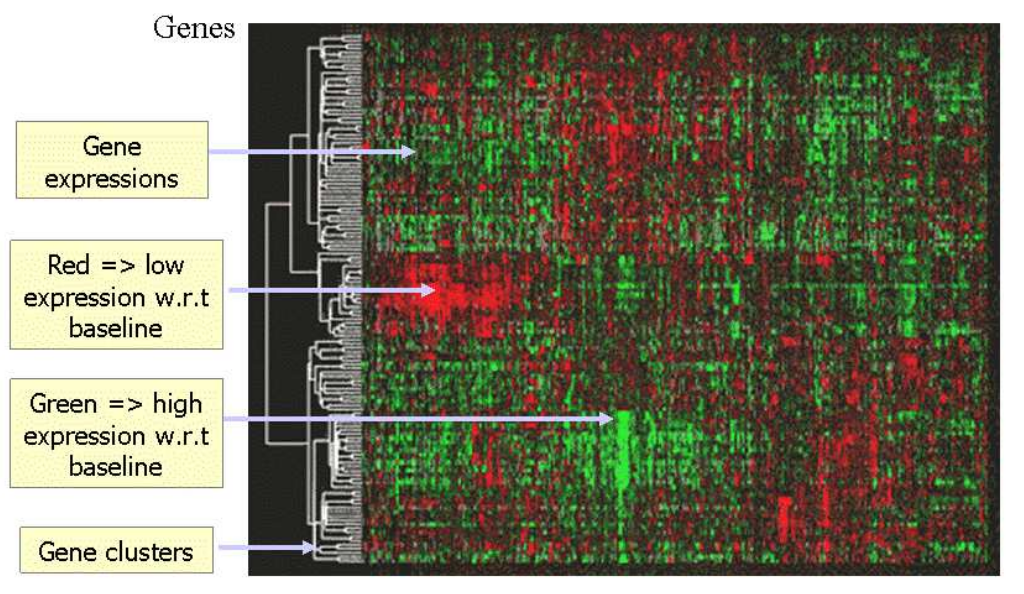
\includegraphics[scale=0.3]{imagenes/c3/Genetica/Genes} 
	\caption{Clustering de genes basado en microarrays. \cite{Survey:2007}}\label{fig:figure13}
\end{figure}

\subsection{Aplicaciones en análisis de textos}

En tareas de clasificación de contenido, el objetivo es dividir de manera automática grandes cantidades de documentos en grupos o clusters. En este caso es posible extraer las restricciones de múltiples recursos auxiliares, por ejemplo, si dos documentos se encuentran en el mismo directorio se podría inferir una restricción de tipo \acf{ML} entre ellos. De esta manera es posible modificar el clustering resultante para que se adapte a un criterio concreto, por ejemplo, crear una jerarquía de documentos semejante a la forma en la que se encuentran organizados en la estructura de directorios de entrada.

\subsection{Aplicaciones en datos web} 

El clustering con restricciones resulta de gran utilidad en el procesado de datos de búsqueda en páginas web. Aquí, el objetivo es agrupar, de manera automática, los resultados de una búsqueda ambigua en el motor de búsqueda en clusters de \acs{URL}s, que se refieran al concepto introducido como consulta en diferentes contextos. En este es posible extraer las restricciones de búsquedas realizadas anteriormente por los usuarios, de manera que se establece una restricción de tipo \acf{ML} entre \acs{URL}s visitadas en la misma sesión de usuario. Aplicar clustering utilizando estas restricciones puede ayudar a sesgar el resultado de las búsquedas hacia las preferencias del usuario.

\subsection{Aplicaciones en datos de audio}

En ciertas tareas de análisis de audio, es posible que no se conozca el número de clases de objetos presentes en los datos, pero las restricciones pueden extraerse directamente del dominio de datos. Esto sucede, por ejemplo, al aplicar clustering para reconocimiento de hablantes en una conversación \cite{BarHillel:2003}. En este caso el número de hablantes no se conoce a priori, pero es fácil detectar si dos hablantes son diferentes o similares y establecer las restricciones en base a ello.

\subsection{Aplicaciones en datos de GPS}

Tal y como se indicó en el inicio e este capítulo, el clustering con restricciones sobre datos \acs{GPS} es utilizado para identificar el carril por el que circula cada vehículo, como se muestra en la figura \ref{fig:figure14} \cite{Wagstaff:2001b}. Cada instancia esta representada por la posición que ocupa el la vía en coordenadas cartesianas bidimensionales $(x,y)$, obtenidas estas en base a los datos \acs{GPS}. La figura \ref{fig:figure15} muestra de manera gráfica esta representación de los datos, cabe destacar que múltiples instancias pueden referirse al mismo vehículo en distintos momentos en el tiempo.

\begin{figure}[!h]
	\centering
	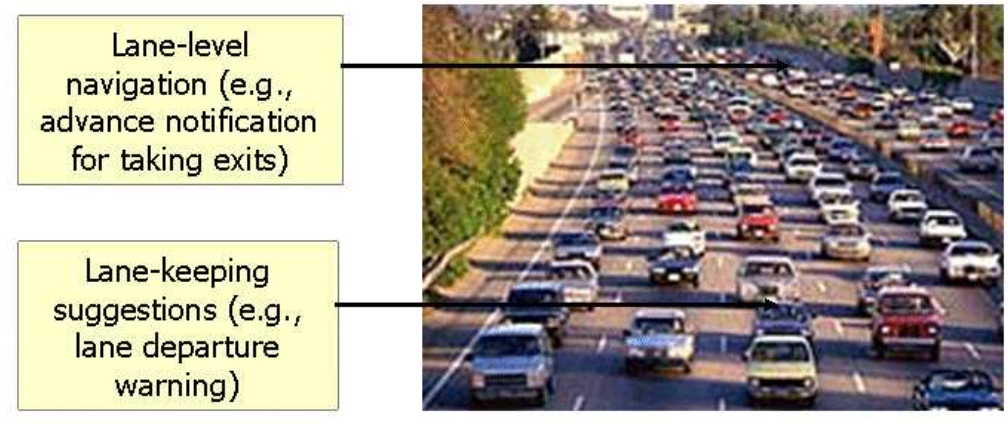
\includegraphics[scale=0.3]{imagenes/c3/GPS/Coches} 
	\caption{Uso de información GPS. \cite{Survey:2007}}\label{fig:figure14}
\end{figure}


En este dominio, los clusters reales tiene forma alargada en el eje horizontal y se encuentran alineados perpendicularmente a la dirección de desplazamiento. Para lograr que los clusters resultantes tengan esta forma, podemos hacer uso de las restricciones. Estableceremos una restricción de tipo \acf{CL} entre aquellas instancias separadas más de 4 metros en dirección perpendicular a la del desplazamiento (ya que los carriles tiene una anchura máxima de 4 metros), y \acf{ML} entre aquellas instancias que presenten continuidad en el eje horizontal, ya que es probable que los vehículos que representan se encuentren en el mismo carril. Este modelo de clustering ha probado ser muy útil en navegación a tiempo real \cite{Wagstaff:2001b}, permitiendo notificar al usuario cuando debe cambiar de carril, o cuando no debe abandonarlo.

\begin{figure}[!h]
	\centering
	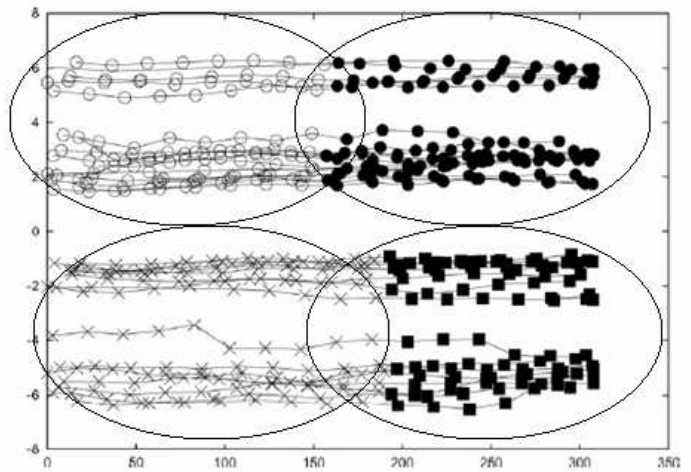
\includegraphics[scale=0.3]{imagenes/c3/GPS/Instancias} 
	\caption{Clusters encontrados en datos GPS sin uso de restricciones. \cite{Wagstaff:2001b} \cite{Survey:2007}}\label{fig:figure15}
\end{figure}

\section{Beneficios del uso de restricciones}

Encontramos dos beneficios principales en el uso de restricciones: (a) incremento de la exactitud en las predicciones de las etiquetas al generar restricciones en base a un subconjunto de instancias etiquetadas, (b) obtención de clusters con geometría adaptable a cada problema. A continuación de discute estos dos beneficios:

Dado un gran conjunto de instancias no etiquetadas $X = \{x_1 \cdots x_u\}$ y $L = \{(x_{u+1}, y_{u+1})\cdots (x_{u+l}, y_{u+l})\}$, un pequeño conjunto de instancias etiquetadas, es común escoger dos elementos de $L$ (con reemplazamiento) y establecer una restricción \acs{ML} entre ellos si pertenecen a la misma clase o, en caso contrario, una de tipo \acs{CL}. Un método apropiado para evaluar los resultados ofrecidos por un método de clustering es medir en nivel de exactitud de este a la hora de predecir las etiquetas del conjunto $X$. Esto normalmente requiere que se especifique el número de clusters deseados igual al número de clases conocidas en $X$ ($k = k*$). Para medir la exactitud se emplean métodos como el \textit{Rand index} \cite{Rand:1971}.

El trabajo de Wagstaff y Cardie \cite{WagstaffCardie:2000}, en el que los autores generaban las restricciones de la manera descrita anteriormente, demostraban que, cuando se realiza un promedio de la exactitud de las predicciones obtenidas con algorimos de clustering con restricciones, variando estas últimas entre experimentos, se obtienen resultados hasta un 20\% mejoras que con las técnicas clásicas.

\begin{observacion}
	
	\textbf{El uso de restricciones, en media, incrementa la precisión.}
	El rendimiento de un método al predecir etiquetas aumenta cuando se promedia empleando numerosos conjuntos de restricciones diferentes.\cite{Survey:2007}
	
\end{observacion}

Esta regla, sin embargo, no es cierta en todos los casos, pues en conjuntos de datos como \textit{Tic-Tac-Toe Endgame}, no se consigue ningún incremento en las predicciones sea cual sea el número de restricciones empleadas. Una explicación dada por los autores es que establecer $k = k*$ no es apropiado en este caso.

El otro beneficio que reportan las restricciones es la posibilidad de obtener clusters con la geometría deseada, un ejemplo ya estudiado en secciones anteriores en este documento es el de aplicar clustering a datos \acs{GPS}.

\section{Problemas del uso de restricciones}




























